\let\negmedspace\undefined
\let\negthickspace\undefined
\documentclass[journal]{IEEEtran}
\usepackage[a5paper, margin=10mm, onecolumn]{geometry}
%\usepackage{lmodern} % Ensure lmodern is loaded for pdflatex
\usepackage{tfrupee} % Include tfrupee package

\setlength{\headheight}{1cm} % Set the height of the header box
\setlength{\headsep}{0mm}     % Set the distance between the header box and the top of the text

\usepackage{gvv-book}
\usepackage{gvv}
\usepackage{cite}
\usepackage{amsmath,amssymb,amsfonts,amsthm}
\usepackage{algorithmic}
\usepackage{graphicx}
\usepackage{textcomp}
\usepackage{xcolor}
\usepackage{txfonts}
\usepackage{listings}
\usepackage{enumitem}
\usepackage{mathtools}
\usepackage{gensymb}
\usepackage{comment}
\usepackage[breaklinks=true]{hyperref}
\usepackage{tkz-euclide} 
\usepackage{listings}
% \usepackage{gvv}                                        
\def\inputGnumericTable{}                                 
\usepackage[latin1]{inputenc}                                
\usepackage{color}                                            
\usepackage{array}                                            
\usepackage{longtable}                                       
\usepackage{calc}                                             
\usepackage{multirow}                                         
\usepackage{hhline}                                           
\usepackage{ifthen}                                           
\usepackage{lscape}
\usepackage{circuitikz}
\tikzstyle{block} = [rectangle, draw, fill=blue!20, 
    text width=4em, text centered, rounded corners, minimum height=3em]
\tikzstyle{sum} = [draw, fill=blue!10, circle, minimum size=1cm, node distance=1.5cm]
\tikzstyle{input} = [coordinate]
\tikzstyle{output} = [coordinate]


\begin{document}

\bibliographystyle{IEEEtran}
\vspace{3cm}

\title{4.6.5}
\author{EE25BTECH11017 - Mahesh Chollangi}
\maketitle
% \newpage
% \bigskip
{\let\newpage\relax\maketitle}

\renewcommand{\thefigure}{\theenumi}
\renewcommand{\thetable}{\theenumi}
\setlength{\intextsep}{10pt} % Space between text and floats


\numberwithin{equation}{enumi}
\numberwithin{figure}{enumi}
\renewcommand{\thetable}{\theenumi}

\textbf{Question}:\\
Find the equation of the line passing through $(2,1,-1)$ and parallel to the line $\vec{r} = (\vec{i} + \vec{j}) + \lambda\brak{2\vec{i} - \vec{j} + \vec{k}}$. Also, find the distance between these two lines.

\solution \\

Let the direction vector of the given line be
\begin{align}
\vec{m} = \myvec{2 \\ -1 \\ 1}
\end{align}

The point through which the required line passes is
\begin{align}
\vec{A} = \myvec{2 \\ 1 \\ -1}
\end{align}

Therefore, the equation of the required line is
\begin{align}
\vec{r}_1 = \vec{A} + \lambda \vec{m} = \myvec{2 \\ 1 \\ -1} + \lambda \myvec{2 \\ -1 \\ 1}
\end{align}

The equation of the given line can be written as
\begin{align}
\vec{r}_2 = \myvec{1 \\ 1 \\ 0} + \mu \myvec{2 \\ -1 \\ 1}
\end{align}

The distance $d$ between two skew lines $\vec{r}_1 = \vec{a}_1 + \lambda \vec{m}$ and $\vec{r}_2 = \vec{a}_2 + \mu \vec{m}$ (with the same direction vector) is given by
\begin{align}
d = \frac{\norm{\brak{\vec{A} - \vec{B}} \times \vec{m}}}{\norm{\vec{m}}}
\end{align}
where $\vec{B} = \myvec{1 \\ 1 \\ 0}$

Compute $\vec{A} - \vec{B}$:
\begin{align}
\vec{A} - \vec{B} = \myvec{2 \\ 1 \\ -1} - \myvec{1 \\ 1 \\ 0} = \myvec{1 \\ 0 \\ -1}
\end{align}

Now, compute the cross product:
\begin{align}
\brak{\vec{A} - \vec{B}} \times \vec{m} 
= 
\begin{vmatrix}
\vec{i} & \vec{j} & \vec{k} \\
1 & 0 & -1 \\
2 & -1 & 1 \\
\end{vmatrix}
\end{align}

Expanding this determinant,
\begin{align}
= \vec{i} \brak{0 \times 1 - (-1) \times (-1)} - \vec{j} \brak{1 \times 1 - (-1) \times 2} + \vec{k} \brak{1 \times (-1) - 0 \times 2} \\
= \vec{i}(0-1) - \vec{j}(1+2) + \vec{k}(-1-0) \\
= -\vec{i} - 3\vec{j} - \vec{k}
\end{align}

Therefore,
\begin{align}
\norm{\brak{\vec{A} - \vec{B}} \times \vec{m}} = \sqrt{1^2 + 3^2 + 1^2} = \sqrt{11}
\end{align}

Now, compute $\norm{\vec{m}}$:
\begin{align}
\norm{\vec{m}} = \sqrt{2^2 + (-1)^2 + 1^2} = \sqrt{4 + 1 + 1} = \sqrt{6}
\end{align}

Thus, the required distance is:
\begin{align}
d = \frac{\sqrt{11}}{\sqrt{6}}
\end{align}

Therefore, the equation of the required line is:
\begin{align}
\vec{r}_1 = \myvec{2 \\ 1 \\ -1} + \lambda \myvec{2 \\ -1 \\ 1}
\end{align}
and the distance between the two lines is
\begin{align}
d = \frac{\sqrt{11}}{\sqrt{6}}
\end{align}
\begin{figure}[H]
    \centering
    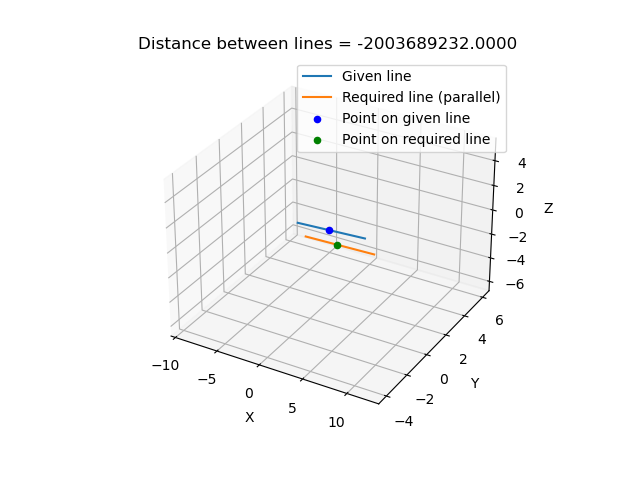
\includegraphics[width=0.8\columnwidth]{Figs/Figure_7.png}
    \caption{3D Plot}
    \label{3D Plot}
\end{figure}
\end{document}